\begin{pastexam}[label={px:df3-110-ds-04}]{地方三等資訊處理 110 年 第四題}
（申論；30 分）

區間堆積（interval heap）是一種優先佇列（priority queue），請回答下列相關的問題。
\begin{itemize}[leftmargin=2.2em]
\item[㈠] 從一個沒有元素的區間堆積開始，依序插入 40, 30, 60, 15, 14, 19, 80, 12, 90 等元素。請畫出最後區間堆積的
樹狀結構圖。（9 分）
\item[㈡] 請自第㈠子題建構的區間堆積中刪除元素 12，並畫出刪除該元素後區間堆積的樹狀結構圖。（3 分）
\item[㈢] 請以一維陣列設計資料結構儲存區間堆積，該資料結構可以透過節點對應之陣列索引值 index 構成的數學式計算出
其父節點 parent、左子節點 left、右子節點 right 與兄弟節點 brother 等在陣列中的索引值。假設此一維陣列之起始索引值
為 0，請列出由 index 構成的計算 parent、left、right、brother 的數學式。並請畫出以此一維陣列儲存第㈠子題建構完成的
區間堆積的結果。（12 分）
\item[㈣] 舉例並說明一既需要提供最高優先元素，也需要提供最低優先元素的優先佇列的應用實例或系統。（6 分）
\end{itemize}
\end{pastexam}

\begin{pastsoln}
答案：㈠ 根 $[12, 90]$；第二層 $[14, 80]$、$[15, 19]$；第三層（都在 $[14, 80]$ 底下）$[30, 40]$、$[60]$。 ㈡ 根
$[14, 90]$；$[30, 80]$、$[15, 19]$；$[30, 80]$ 底下 $[40, 60]$。 ㈢ $\mathit{parent} = \lfloor(\mathit{index}-1)/2\rfloor$、
$\mathit{left} = 2\,\mathit{index} + 1$、$\mathit{right} = 2\,\mathit{index} + 2$、$\mathit{brother} = \mathit{index} + 1$
（奇數）或 $\mathit{index} - 1$（偶數）。 ㈣ 例如交易撮合、有容量上限的排程佇列。

\textbf{區間堆積的定義}（資結書第~8.5.4~節）：一棵完整二元樹，每個節點放兩個元素 $a \le b$，看成區間 $[a, b]$；最後一個
節點可以只放一個元素。 每個節點的區間都\textbf{包含}它子節點的區間（只有一個元素的節點看成單點區間）。 因此左端點
構成一個最小堆積、右端點構成一個最大堆積，根的 $a$ 是最小值、$b$ 是最大值。

\textbf{插入 $x$}（Sahni 的做法）：
\begin{itemize}
\item 若最後一個節點只有一個元素，$x$ 放進這個節點，和原有元素排成 $[\min, \max]$；否則新開一個節點只放 $x$。
\item 設父節點是 $[a, b]$。 若 $x < a$，$x$ 沿著\textbf{左端點}往上浮（像最小堆積：父節點的左端點比 $x$ 大就搬下來）；
若 $x > b$，沿著\textbf{右端點}往上浮（像最大堆積）；若 $a \le x \le b$，結束。
\end{itemize}
節點依層序編號 $0, 1, 2, \ldots$（節點 $k$ 的子節點是 $2k+1$、$2k+2$）。
\begin{center}
\small
\begin{tabular}{l>{\raggedright\arraybackslash}p{0.42\linewidth}>{\raggedright\arraybackslash}p{0.40\linewidth}}
\toprule
插入 & 過程 & 結果（節點 $0, 1, 2, \ldots$） \\
\midrule
40 & 空堆積，開節點 0 & $[40]$ \\
30 & 節點 0 只有一個元素，放進去 & $[30, 40]$ \\
60 & 開節點 1；$60 > 40$，$40$ 搬下來 & $[30, 60]$, $[40]$ \\
15 & 放進節點 1 成 $[15, 40]$；$15 < 30$，$30$ 搬下來 & $[15, 60]$, $[30, 40]$ \\
14 & 開節點 2；$14 < 15$，$15$ 搬下來 & $[14, 60]$, $[30, 40]$, $[15]$ \\
19 & 放進節點 2 成 $[15, 19]$；在 $[14, 60]$ 內，結束 & $[14, 60]$, $[30, 40]$, $[15, 19]$ \\
80 & 開節點 3（父 1）；$80 > 40$，$40$ 下來；$80 > 60$，$60$ 下來 & $[14, 80]$, $[30, 60]$, $[15, 19]$, $[40]$ \\
12 & 放進節點 3 成 $[12, 40]$；$12 < 30$，$30$ 下來；$12 < 14$，$14$ 下來 & $[12, 80]$, $[14, 60]$, $[15, 19]$, $[30, 40]$ \\
90 & 開節點 4（父 1）；$90 > 60$，$60$ 下來；$90 > 80$，$80$ 下來 & $[12, 90]$, $[14, 80]$, $[15, 19]$, $[30, 40]$, $[60]$ \\
\bottomrule
\end{tabular}
\end{center}
（插入 $12$ 時 $12$ 成為節點 3 的左端點，沿左端點往上：節點 1 的左端點 $30 > 12$，搬到節點 3；根的左端點 $14 > 12$，搬到
節點 1；$12$ 到根。）

\textbf{㈠ 最後的區間堆積}：
\begin{center}
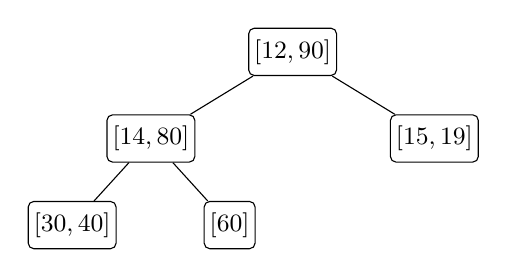
\begin{tikzpicture}[v/.style={rectangle,rounded corners=2pt,draw,minimum height=6mm,inner sep=2pt,font=\small},
  level distance=11mm, level 1/.style={sibling distance=36mm}, level 2/.style={sibling distance=20mm}]
\node[v] {$[12, 90]$}
  child {node[v] {$[14, 80]$} child {node[v] {$[30, 40]$}} child {node[v] {$[60]$}}}
  child {node[v] {$[15, 19]$}};
\end{tikzpicture}
\end{center}
檢查：$[14, 80] \subseteq [12, 90]$，$[15, 19] \subseteq [12, 90]$，$[30, 40]$ 和 $60$ 都在 $[14, 80]$ 內。

\textbf{㈡ 刪除 $12$}：$12$ 是根的左端點，也就是最小值，做「刪除最小值」：拿出最後一個節點的左端點 $p$（這裡最後一個
節點只有 $60$，取出後節點 4 消失），從根開始沿左端點往下找位置：
\begin{enumerate}
\item 根的左端點空出來。 子節點的左端點是 $14$、$15$，較小的 $14 < 60$，$14$ 上到根，洞移到節點 1（右端點 $80$）。
$60 \le 80$，不用和右端點交換。
\item 節點 1 的子節點只剩節點 3，左端點 $30 < 60$，$30$ 上來，洞移到節點 3（右端點 $40$）。 $60 > 40$，交換：$40$
變成要放的值，$60$ 留在節點 3 的右端點。
\item 節點 3 沒有子節點，$40$ 放進左端點：節點 3 成為 $[40, 60]$。
\end{enumerate}
\begin{center}
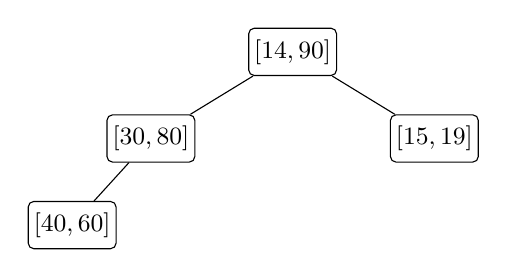
\begin{tikzpicture}[v/.style={rectangle,rounded corners=2pt,draw,minimum height=6mm,inner sep=2pt,font=\small},
  level distance=11mm, level 1/.style={sibling distance=36mm}, level 2/.style={sibling distance=20mm}]
\node[v] {$[14, 90]$}
  child {node[v] {$[30, 80]$} child {node[v] {$[40, 60]$}} child[missing] {}}
  child {node[v] {$[15, 19]$}};
\end{tikzpicture}
\end{center}
新的最小值 $14$ 在根；$[40, 60] \subseteq [30, 80] \subseteq [14, 90]$。 （區間堆積和資結書第~8.5.3~節的 SMMH 一一對應：
SMMH 去掉空的根、每對兄弟合成一個節點就是區間堆積，用 SMMH 的插入和刪除會得到相同的結果。）

\textbf{㈢ 陣列表示}。 用一維陣列 $H[0..m-1]$，依層序存放節點，每一格是一個節點，含兩個欄位 $\mathit{low}$（左端點）、
$\mathit{high}$（右端點）；另記元素總數 $n$，節點數 $m = \lceil n/2 \rceil$，$n$ 為奇數時最後一格只用 $\mathit{low}$。
節點索引 $\mathit{index}$ 從 $0$ 開始：
\begin{align*}
\mathit{parent} &= \left\lfloor \frac{\mathit{index} - 1}{2} \right\rfloor \quad (\mathit{index} \ge 1), \\
\mathit{left} &= 2 \cdot \mathit{index} + 1, \qquad \mathit{right} = 2 \cdot \mathit{index} + 2, \\
\mathit{brother} &= \begin{cases} \mathit{index} + 1, & \mathit{index} \text{ 為奇數（左子節點）}, \\
\mathit{index} - 1, & \mathit{index} \text{ 為偶數且} \ge 2 \text{（右子節點）}, \end{cases}
\end{align*}
算出的索引 $\ge m$ 表示不存在。 ㈠ 的結果：
\begin{center}
\small
\begin{tabular}{l*{5}{|c}|}
\cline{2-6}
index & 0 & 1 & 2 & 3 & 4 \\ \cline{2-6}
low & 12 & 14 & 15 & 30 & 60 \\ \cline{2-6}
high & 90 & 80 & 19 & 40 & \\ \cline{2-6}
\end{tabular}
\end{center}
例如 $\mathit{index} = 3$：parent $= 1$、brother $= 4$、left $= 7$（不存在）。

若規定陣列每格只能放一個整數，也可以把節點 $k$ 的兩端放在 $B[2k]$、$B[2k+1]$：
$B = \langle 12, 90, 14, 80, 15, 19, 30, 40, 60 \rangle$。 這時元素 $x$ 所在的節點是 $k = \lfloor x/2 \rfloor$，同一端
在父節點、左子、右子、兄弟節點的位置分別是 $2\lfloor (k-1)/2 \rfloor + (x \bmod 2)$、$2(2k+1) + (x \bmod 2)$、
$2(2k+2) + (x \bmod 2)$、$x \pm 2$（$k$ 奇數取 $+$，偶數取 $-$）。

\textbf{㈣ 應用}（雙端優先佇列，最高、最低都要能取）：
\begin{itemize}
\item \textbf{交易撮合}：證券或拍賣系統裡，買方出價要能隨時取出\textbf{最高}的、賣方要價要能取出\textbf{最低}的來撮合；
同一個委託簿還要能撤掉偏離市價最遠的單。
\item \textbf{容量有限的排程佇列}：例如網路路由器的封包緩衝區或伺服器的工作佇列，平時取出優先權\textbf{最高}的處理；
緩衝區滿了又有新工作進來時，要丟掉優先權\textbf{最低}的那一個。 一般的堆積只能快速處理其中一端，區間堆積兩端都是
$O(\log n)$。
\item 其他：外部排序時用它保存「中間」那批資料（每次把最小或最大的移出）；只保留前 $k$ 名的排行榜，新資料進來時和
最低的比、要公布時取最高的。
\end{itemize}
\end{pastsoln}
